% begin module diff-eq-logistic-graph
\begin{frame}
\[
\frac{\diff P}{\diff t} = kP\left( 1 - \frac{P}{K}\right)
\]
\begin{itemize}
\item  What do the solutions look like?
\item<2->  $P = 0$ and $P = K$ are special solutions, called equilibrium solutions.
\item<3->  If $P > K$, then $1 - P/K < 0$ , so $\diff P/ \diff t < 0$, and $P$ decreases.
\item<4->  If $P < K$, then $1 - P/K > 0$, so $\diff P/\diff t > 0$, and $P$ increases.
\item<5->  As $P \rightarrow K$, $1 - P/K \rightarrow 0$, so $\diff P/\diff t \rightarrow 0$ and $P$ levels off.
\end{itemize}
\begin{center}
\ \only<handout:0| -1>{%
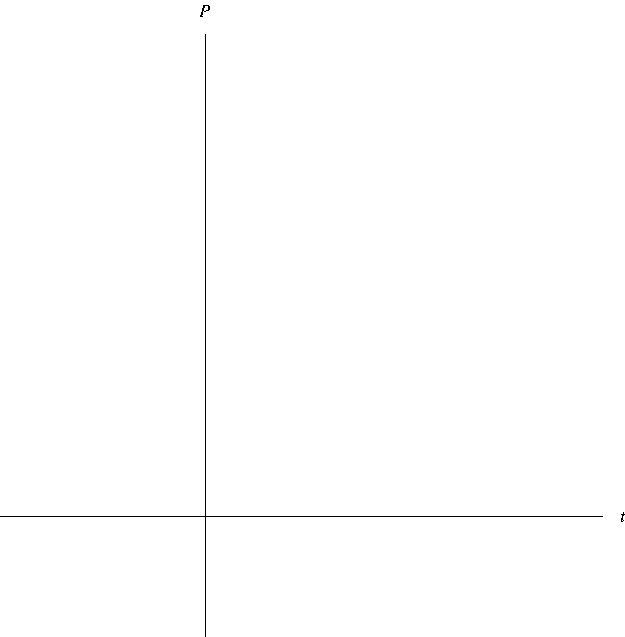
\includegraphics[height=4cm]{diff-eq-models/pictures/10-01-logistica.pdf}%
}%
\only<handout:0| 2>{%
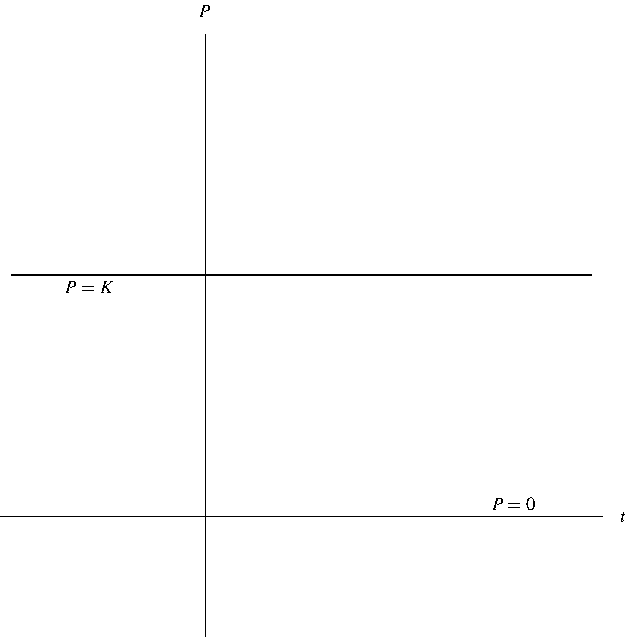
\includegraphics[height=4cm]{diff-eq-models/pictures/10-01-logisticb.pdf}%
}%
\only<handout:0| 3-4>{%
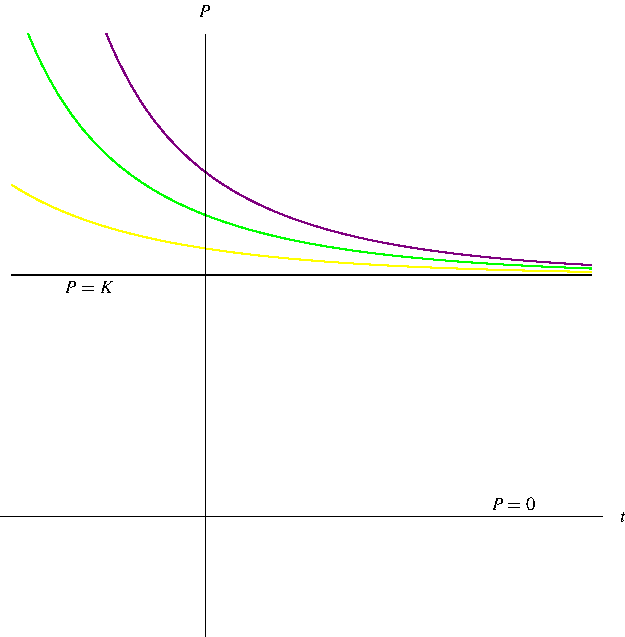
\includegraphics[height=4cm]{diff-eq-models/pictures/10-01-logisticc.pdf}%
}%
\only<5->{%
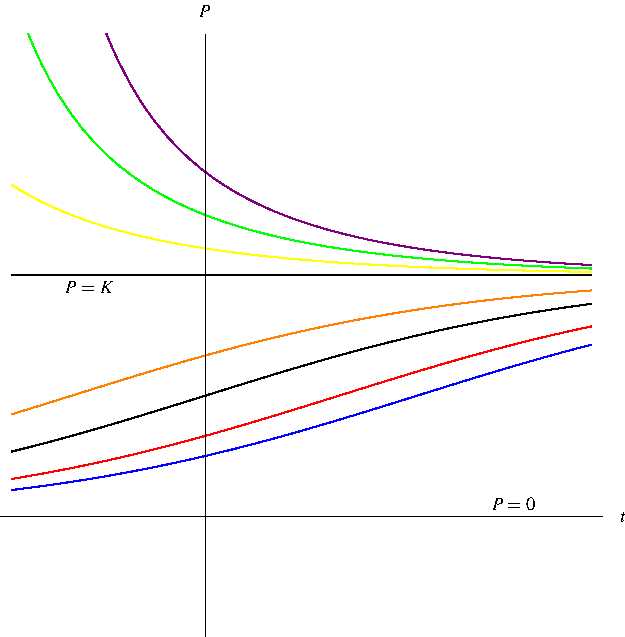
\includegraphics[height=4cm]{diff-eq-models/pictures/10-01-logisticd.pdf}%
}%
\end{center}
\end{frame}
% end module diff-eq-logistic-graph
